% Set the author and title of the compiled pdf
\hypersetup{
  pdftitle = {\Title},
  pdfauthor = {\Author}
}

In Semester One, of this course we covered zero and non-zero sum games (Nash
games) and search algorithms to find equlibriums (minimax and alpha beta
pruning). In this semester, we are no longer assuming that each player has the
same `role' and that the games are zero-sum. We are letting there be an infinite
number of positions for each player to take and not assuming that players have
perfect information.

We're going to be looking at Stackelberg games; an example of which could be
retail pricing. Different firms might offer different prices on products, they
can choose a price from an infinate set (the real numbers) and some firms might
have private information that others might not\footnote{Typical examples of
unknown information include payoff functions or unit cost.}.

An industry can be controlled or dominated by a one, two or multiple entities:

\begin{description}
  \item \textbf{Monopoly}: When an industry consists of a single firm.
  \item \textbf{Duopoly}: When an industry consists of two firms.
  \item \textbf{Oligopoly}: When an industry consists of a few firms (and when
  each decision one takes impacts on the other's profits).
\end{description}

In duopoly/oligopoly situations, the roles of the players are different. If one
firm chooses to change its prices first, then the others have to decide what to
do in light of the change; and may not know the full economic and/or political
motivations behind the initial move.

In a two player Stackelberg game, one player selects his strategy first, and
then the other responds. The first player is called the leader ($P_L$) and the
second is called the follower ($P_F$). This contrasts with Nash games, where all
of the players select their strategies simultaneously.

Both the leader and follower have payoff functions\footnote{A payoff function
indicates the benefit for that player given the chosen strategies of all the
players.}, which they want to maximise:

\[
  \begin{split}
  &J_L(U_L, U_F)\\
  &J_F(U_L, U_F)
  \end{split}
\]

A strategy space is the set of all possible strategies for a single player. The
leader's strategy space is $U_L$ and the follower's is $U_F$. They can include
finite (discrete) or infinite (continuous) strategies. To play the game, the
leader must first choose some strategy $u_L \in U_L$ and then the follower must
choose some strategy $u_F \in U_F$.

In a Stackelberg game, when the leader has announced $u_L$, the follower selects
a strategy using their reaction function $R(u_L) \in U_F$ such that:

\[
  J_F(u_L, R(u_L)) = MAX_{u_F \in U_F} J_F(u_L, u_F)
\]

This looks complicated, but what it says is that the payoff for the follower is
given the parameters $u_L$ and $u_F$. The follower obviously wants to maximise
their payoff, and so tries to find the strategy $u_F \in U_F$ that will maximise
their payoff. This isn't always easy, since enumerating every possible strategy
and knowing what will happen if any given strategy is deployed is sometimes
impossible.

In order to solve a Stackelberg game, we need to solve the following problem:

\begin{itemize}
  \item What is the follower's reaction function $R(u_L)$?
  \item When we've found that, what leader strategy $u_L$ maximises the leader's
  payoff function:
  \[
    J_L(u^*_L, R(u^*_L)) = MAX_{u_L \in U_L} J_L(u_L, u_F)
  \]
\end{itemize}

If the follower has a reaction function $R(u_L)$ and there exists a leader
strategy $u^*_L \in U_L$ and the response strategy is $u^*_F = R(U^*_L) \in U_F$
such that $J_L(u^*_L, u^*_F) = MAX_{u_L \in U_L} J_L(u_L, R(u_L))$, then
$(u^*_L, u^*_F)$ is called a \textbf{Stackelberg strategy/equilibrium}; i.e.
both sides are paying an optimal strategy.

We always assume that the follower is rational and tries to find the best
reaction strategy. Sometimes this is untrue, for example if taking a non-optimal
strategy results in a rival player having a big loss.

For a player to be a leader, he needs to act first. There is no requirement that
they are a leader in an economic or political sense. The only requirement to be
a follower is to react to the leader's strategy\footnote{Note that this does not
mean the follower is in a weaker position.}. As mentioned before, Stackelberg
games can be continuous or discrete, depending on if the strategy space is
finite or infinite.

Since the only difference between a Nash game and a Stackelberg game is whether
moves are played simultaneously or in order, should we prefer Nash or
Stackelberg games? If the player has the opportunity to be the leader, then
Stackelberg games should be preferred, since he will always be better off than
in a Nash game in this instance. Here's a mini-proof:

Let $u_1$ and $u_2$ be the strategies for player's one and two, and let
$J_1(u_1, u_2)$, $J_2(u_1, u_2)$ be their respective payoff functions. If there
is a Stackelberg strategy and a Nash strategy, then:

\[
  J_1(u^{Stackelberg}_1, u^{Stackelberg}_2) \geq J_1(u^{Nash}_1, u^{Nash}_2)
\]

Note that sometimes the follower can be better off in a Stackelberg game, but
the leader would still be better off playing the Stackelberg game than playing a
Nash game. Other times, the player could win as the leader or follower, but win
better as the follower.

For the follower to play the game, he needs to know nothing about the leader or
his strategy space. However, for the leader to play, he needs to know the
follower's payoff function and strategy space in order to work out the action
that will give the max payoff. If such information is not available, then the
leader must guess or learn it (based off previous experience or data).

% Lecture 2

\section{Solving Stackelberg game problems}

We can solve with two sequential maximisation problems, each for a single
player:

\begin{enumerate}
  \item For each of the leader's strategies $u_L \in U_L$, solve:
    \[
      max_{u_F \in U_F}(J_F(u_L, u_F)
    \]
    The solution for this is the follower's reaction function $R(u_L)$.
  \item Find the best strategy for the leader by solving:
    \[
      max_{u_L \in U_L}(J_L[u_L, R(u_L)])
    \]
    If $u^*_L$ is the strategy found in the above maximisation, and
    $u^*_L = R(u^*_L)$, then ($u^*_L, u^*_F)$ is a Stackelberg strategy.
\end{enumerate}

So, in order to find the Stackelberg strategy, we need to solve two maximisation
problems. This is A-level maths, but we can recap it in the next bit.

\subsection{How to find the maximum point of a function over a continuous space}

We want to find a point $x^* \in X$ that maximises $f(x)$ over $X$, such that
$\forall x \in X, f(x^*) \geq f(x)$. Such a point is called the global maximum
point of $f(x)$ on $X$. A local maximum point $y^*$ is the maximum value of
$f(x)$ within the region $X$, such that $\forall x \in X, f(y^*) \geq f(x)$.

\begin{figure}
  \centering
  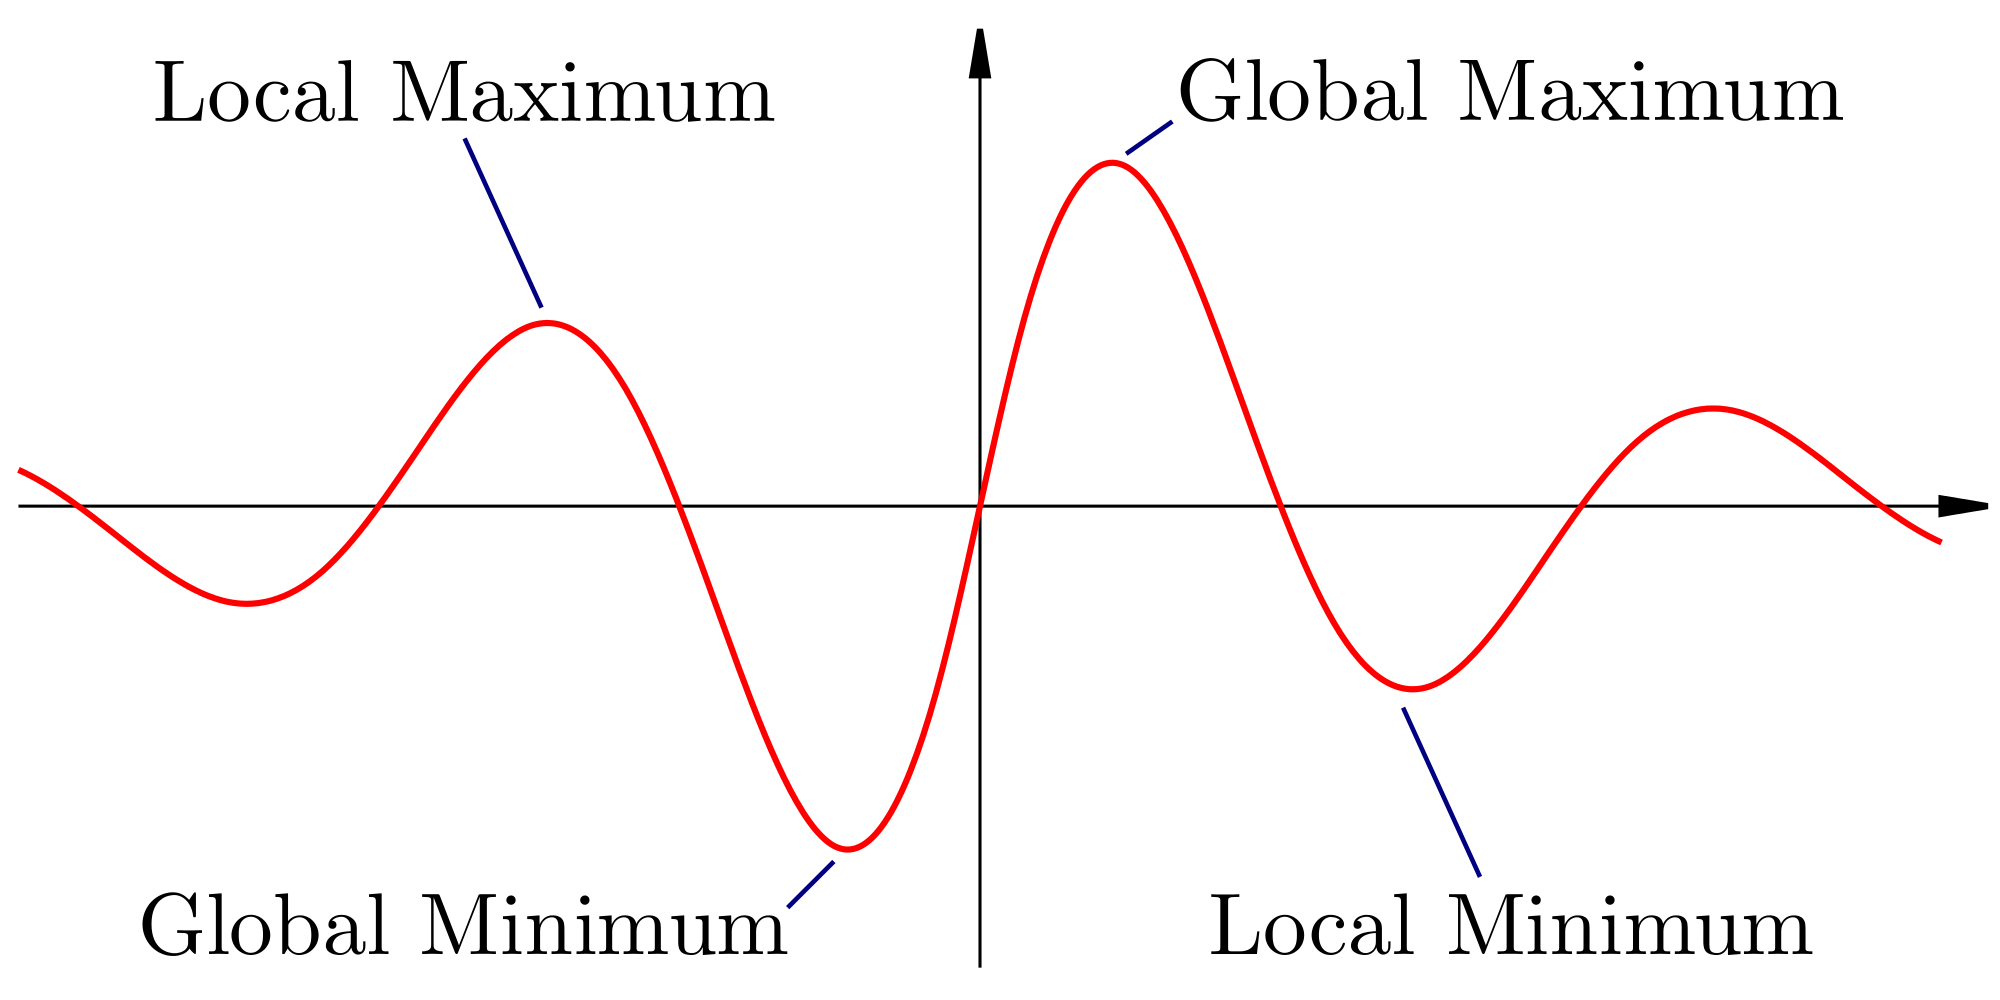
\includegraphics[width=\textwidth]{images/maxima}
  \caption{Wikipedia's pictorial explanation of minima and maxima.}
  \label{fig:maxima}
\end{figure}

The standard method for trying to find a maximum of a function is by using
derivatives. A derivative is usually notated by a dash after the function.
Finding the derivative of a derivative is called the second order derivative
function, and has two dashes.

A first order derivative represents the gradient of the line drawn by the
function at a specific point. If $f'(x) > 0$, then the line slopes upwards, and
if $f'(x) < 0$ then it's sloping down. Obviously if it is equal to zero, then
the line is horizontal.

\marginpar{Question: Is this finding derivitives linear time? I think that you'd
parse the input function into an AST\footnote{Abstract Syntax Tree}
(linear time) with an LL(1) grammar, then repeatedly apply rules for
finding the derivative (which is probably poly-time).}

\subsubsection{Calculating a derivative}

The most simple rule is:

\[
  f(x) = x^n \therefore f'(x) = nx^{n-1}
\]

This means if the function is constant, it disappears:

\[
  f(x) = C \therefore f'(x) = 0
\]

Here are three simple examples:

\[
  f(x) = x^2 \therefore f'(x) = 2x
\]

\[
  f(x) = x^3 \therefore f'(x) = 3x^2
\]

\[
  f(x) = 5 \therefore f'(x) = 0
\]

If a function is composed of other functions that are added together (of the
form $f(x) = f_1(x) + \dots + f_n(x)$ then:

\[
  f'(x) = f_1'(x) + \dots + f_n'(x)
\]

Just like:

\[
  f(x) = -2x^2 + 4x + 5 \therefore f'(x) = -4x + 4
\]

Finally, if it's composed of functions that are multiplied together, then
$f'(x)= f_1'(x)f_2(x) + f_1(x)f_2'(x)$:

\[
  f(x) = x^2 \times x \therefore
    f'(x) = [x^2]' \times x + x^2 \times [x]' = 2x \times x + x^2 \times 1
          = 2x^2 + x^2 = 3x^2
\]

\subsubsection{Finding maxima}

Once you've found the derivative of your function, and then found the points
where the derivatives are 0 (and the gradient of the line is therefore zero),
you need to determine whether that point is a minima or maxima. To do this, we
differentiate again to get the second order derivative. If the value of $f''(x)
\geq 0$ then the gradient is increasing, therefore it's a minima. Because of
this, we want points where the second order derivative gives a negative value,
indicating that the point is a maxima.

To find the largest maxima, we simply find the one that is largest value of
$f(x)$.

% Lecture 3

\section{Solving Stackelberg game problems}

We know that there are two steps to solve a Stackleberg game; first of all, you
must solve the maximisation problem $\text{max}{u_F\in U_F}J_F(u_L,u_F)$, giving
the reaction function $R(u_L)$. Then you must find the best leader strategy by
solving $\text{max}_{u_L \in U_L} J_L(u_L, R(u_L))$ such that $(u_L, u_F)$ is
the Stackelberg strategy.

The strategy space (i.e. the different prices that the leader and follower can
set) is $U_L = [c_L, +\infty], U_F = [c_F, +\infty]$, where $c_L, c_F$ are the
cost of each unit for the leader and follower respectively.

The payoff function (i.e. how much profit the leader and follower make) is
defined by:

\[
  J_L(u_L, u_F) = (u_L - c_L) \times S_L(u_L, u_F)
\]

\[
  J_F(u_L, u_F) = (u_F - c_F) \times S_F(u_L, u_F)
\]

This is essentially the profit per unit (sale price minus cost) multiplied by
the number of units sold in the sale. The sale function is given to you in exam
questions and is a quadratic function over $u_L$ and $u_F$.

We want to find the optimal values for $u_L$ and $u_F$. To do this, we
first differentiate $J_F$., then we differentiate $J_L$ and sub in the
value for $u_F$ we found in the first stage so we can get
answers. Lets do an example; given the following situation, we want to
find the follower's reaction function, and then an optimal values for
$u_L$ to give us maximum profit:

\[
  J_L(u_L, u_F) = (u_L - c_L) \times S_L(u_L, u_F)
\]

\[
  J_F(u_L, u_F) = (u_F - c_F) \times S_F(u_L, u_F)
\]

\[
  c_F = 1 = c_F
\]

\[
  S_L =  5 - 2u_L + u_F
\]

\[
  S_F = 6 + u_L - 2u_F
\]

To get the reaction function, we differentiate $J_F$:

\[
  \begin{split}
    0 &= \frac{d}{du_F}J_F(u_L,u_F)\\
      &= \frac{d}{du_F}(u_F - 1)(6 + u_L - 2u_F)\\
      &= \frac{d}{du_F}6u_F + u_Fu_L - 2u_F^2 - 6 - u_L + 2u_F\\
      &= u_L - 4u_F + 8
  \end{split}
\]

If we differentiate again, we see that this is a maxima ($-4 > 0$).

We can rearrange it so that: $J_f'(U_L,U_F) = R(u_L) = \frac{u_L}{4} + 2$.

Now we can sub in the value for $u_F$ into $J_L$:

\[
  \begin{split}
    J_L(u_L, R(u_L)) &= (u_L - 1)(5 0 2u_L + R(u_L))\\
                     &= \frac{1}{4}(35u_L - 7u_L^2 - 28)
  \end{split}
\]

And differentiate:

\[
  \frac{d}{du_L}J_L(u_L, R(u_L)) = \frac{1}{4}(35 - 14u_L) = 0
\]

If we rearrange that, we get $u_L = \frac{35}{14}$, therefore $u_F =
2.625$, which are the optimum values of $U_L$ and $U_F$ in terms of
the leader profit.

This means the profits are:

\[
  J_L(\frac{35}{14}, 2.625) = (\frac{35}{14} - 1)(5 - 2\frac{35}{14} + 2.625) = 3.9375
\]

\[
  J_F(\frac{35}{14}, 2.625) = (2.625 - 1)(6 + \frac{35}{14} - 2(2.625)) = 5.28125
\]

%Lecture 4

\section{Stackelberg games with imperfect information}

It is very rare that both players in a two person Stackelberg game will have
perfect information; in any case, it is in their interest to hide information
from one-another. In a game of imperfect information, the follower is not
affected; their job is the same (respond to whatever the leader does).

However, this is a huge change for the leader. Without knowing the strategy
space for the follower, or the follower's reaction function, they can't work out
a good strategy. We need to come up with a technique to let the leader `guess' a
good strategy based of what we \textit{do} know about the game.

There are two obvious solutions, and one machine learning solution to this.
We're interested in the ML solution, but the obvious solutions are:

\begin{itemize}
  \item Choose to be the follower. Then we don't have to decide on the first
  strategy, and can just choose a reaction. However, this isn't always possible
  (sometimes you're forced to move first).
  \item Find the best strategy for the worst scenario; that is to say we should
  find the best, worst strategy:
  \[
    u_L = arg max_{u_L \in U_L}(min_{u_F \in U_F}J_L(u_L, u_F))
  \]
  Though this gives a lower bound on the payoff, it is also far too
  conservative. Imagine if you always planned for the worst and never considered
  (never mind hoped) for the best!
\end{itemize}

However, the best solution is to attempt to learn what the follower will do
based on what has happened in the past. Many two person Stackelberg games are
played repeatedly (e.g. setting oil prices every day), and therefore there is a
lot of information available to learn from. All we need to learn is the
follower's reaction function; i.e. what value they will choose for $u_F$ given
any chosen $u_L$.

The approach we're going to use to do this is called linear regression. This
involves finding a linear function that gives similar values to what the
follower has done in the past. You could also use a polynomial function, a
neural network (neural networks are called the \textit{universal approximation},
since they can mimic any function), or many other different techniques.

So, if $y = R(x)$ be the unknown function, and imagine we have a set of $T$
datapoints where we know the input $x$ and the value $y$. We want to make a new
function $\hat{R}(x)$ that will approximate $R(x)$.

We define $\epsilon(x) = R(x) - \hat{R}(x)$, and try to make
$\epsilon$ as small as possible for all values of $x$. Unfortunately,
since we don't know $R$, we can't work out $\epsilon$. However, we can
work out the value of $\epsilon$ for all the datapoints we do
have. Making the following function (called the least square
criterion) as small as possible is the aim of the regression:

\[
  \sum^T_{t=1}\epsilon^2[x(t)] = \sum^T_{t=1}\left(y(t) - \hat{R}(x(t))\right)^2
\]

Designing a function is problem dependent, but we know our reaction
function will be linear (because we're not considering other functions
in the course):

\[
  R(x) = a + bx
\]

To make $\hat{R}(x)$ imitate $R(x)$, we must find values for $a$ and $b$ that
minimise the squared criterion we had before:

\[
  min_{a,b} \sum^T_{t=1}\left(y(t) - (a + b x(t)))\right)^2
\]

Instead of solving the minimising problem, we can instead solve the following
maximisation problem:

\[
  max_{a,b} - \sum^T_{t=1}\left(y(t) - (a + b x(t)))\right)^2
\]

We can use partial differentiation to do this (just like in
\texttt{COMP36212}), but it's tricky, so this is what you will eventually get:

\[
  a = \frac{ \sum^T_{t=1}x^2(t)\sum^T_{t=1}y(t)
    - \sum^T_{t=1}x(t)\sum^T_{t=1}x(t)y(t) }{ T\sum^T_{t=1}x^2(t) -
    (\sum^T_t{=1}x(t))^2 }
\]

\[
  b = \frac{
    T\sum^T_{t=1}x(t)y(t) - \sum^T_{t=1}x(t)\sum^T_{t=1}y(t)
  }{
    T\sum^T_{t=1}x^2(t) - (\sum^T_t{=1}x(t))^2
  }
\]

% Lecture 5

\section{Multivariable regression}

Now we know how to solve a linear regression problem with one variable, but
often, there isn't just one variable. If there are three fuels in a petrol
station (diesel, unleaded, super unleaded), then there will be three variables,
and we want to learn strategies for all of them.

Here, the leader \& follower strategies will be:

\[
  u_L = (u^L_1, u^L_2, u^L_3)
\]

\[
  u_R = (u^R_1, u^R_2, u^R_3)
\]

The follower's reaction function is:

\[
\hat{R}(u_L) = \hat{A} + \hat{B} u_L
  \begin{bmatrix}
    \hat{a}_1\\
    \hat{a}_2\\
    \dots\\
    \hat{a}_f\\
  \end{bmatrix}
  +
  \begin{bmatrix}
    \hat{b}_{1,1}& \hat{b}_{1,2} & \dots & \hat{b}_{2,n_L}\\
    \hat{b}_{2,2}& \hat{b}_{2,2} & \dots & \hat{b}_{2,n_L}\\
    \dots & \dots & \dots & \dots\\
    \hat{b}_{n_f,1} & \hat{b}_{n_f,2} & \dots & \hat{b}_{n_f,n_L}\\
  \end{bmatrix}
  \begin{bmatrix}
    \hat{u}_1^L\\
    \hat{u}_2^L\\
    \dots\\
    \hat{u}_{n_L}^L\\
  \end{bmatrix}
\]

Given the leader's strategy ($u_L$), the follower will react using:

\[
  \hat{R}_i(u_L) = \hat{a}_i + \sum^{n_L}_{j=1}\hat{b}_{i,j}u^L_{j}
\]

In essence, we're trying to find the mathematical relationship between an output
variable and several input variables. All of them take continuous values (if the
dependent is discrete, then it's a classification problem). Such problems are
widely used in prediction and forecasting.

The idea is that we want to find values for $\theta$ that we can sub into
$\hat{R}$, such that:

\[
  \begin{split}
  \theta^* &= arg~min_\theta \sum^T_{t=1}\epsilon^2(t)\\
           &= arg~min_\theta \sum^T_{t=1}(R[X(t)] - \hat{R}[X(t), \theta])^2\\
           &= arg~min_\theta \sum^T_{t=1}(y(t) - \hat{R}[X(t), \theta])^2
  \end{split}
\]

Since $\hat{R}(X, \theta) = (1, x_1 \dots, x_n) \left( \begin{smallmatrix}
a_0\\ a_1\\ \dots \\ a_n \end{smallmatrix} \right) = a_0 + a_1x_1 + \dots +
a_nx_n$, we just need to find a solution to:

\[
  \theta^* = arg~min_\theta \sum^T_{t=1}(y(t) - [a_0 + a_1x_1(t) + \dots +
a_nx_n(t)])^2
\]

Where $\theta = (a_0, a_1, \dots, a_n)$.

% Cont from slide 16, lecture 5

% Lecture 6

\section{Learining in games}

There are two types of Stackelberg strategy generators; online and offline ones.
In offline learning, the reaction function is regarded as a linear regression
problem, and is solved by applying the least square method to the historical
data. All the learning is done before the playing starts.

In online learining, we aim to carry on learning even while the game is being
played. The reaction strategy from the follower is updated as we play the game.
We need to work out how to incorperate the follower's moves into our strategy.

The reason why online methods are preferred, is that the environment in which
the game is played is always changing; costs may change, share prices may change
etc. The follower's reaction function will change over time to reflect this.

There are two commonly used methods:

\begin{description}
  \item \textbf{Moving Window Approach}:\\
    Here, we only consider $n$ historical points, and as new data comes in, we
    discard old data.
    %TODO: Expand that ^^
    To make it better, we can add a parameter $\lambda$ to make old datapoints
    mean less than new ones. The impact of the $n$th most recent datapoint is
    $n \times \lambda ^{n-1}$, and $\lambda \approx 0.95-0.99$.
  \item \textbf{Recursive Least Square Approach}:\\
    
\end{description}

% Lecture 7

\section{Mechanism Design}

Mechanism design involves taking an engineering approach to designing
economic mechanisms or incentives in order to steer the outcome of
events/transactions/games etc towards a desired objective. As with the
Nash games in semester one, and the Stackleberg games in the first
part of semester two, it is always assumed that the players will act
rationally. Since we start from the desired outcomes, and design a
game to produce these outcomes, mechanism design is also known as
\textit{reverse game theory}.

\subsection{A toy example}

A simple example is that of a mother dividing a cake for her two
children, with a view to them both getting exactly half since
otherwise they will complain. If the mother cuts the cake as equally
as she can, then there is a risk that one or both of the children will
have a different view on the size of the pieces to her, and will want
a specific piece.

\marginpar{Think about how this would work for $n$ children.}

The solution is to have one child cut the cake into two pieces, but
then let the other child have first pick of the pieces. Then, no
matter if the first child cuts the cake evenly or not, the second
child will take whichever one that they think is biggest, and since
the first child cut the cake in the first place, they shouldn't (in
theory) contest the choice.

\subsection{A real example}

There are lots of more interesting examples of mechanism design, such
as the government assigning licences to mobile operators. If we view
the government as one player, and the different mobile operators as
$n$ different players, then it is easy to see their differing aims.
The government wants to allocate a licence to whoever values it the
most highly since an operator who highly values the licence is likely
to use it best for their customers and maximise \textit{social
surplus}. The goal of mobile operators is to maximise their own profit
(i.e. to minimise the price they actually pay for the licence).

If the government could simply ask for an honest reccommendation of
each mobile operator's valuation of the licence, then they could
simply give the licence to the highest valuing operator. However,
since the government does not know the \textit{true} valuation (as
opposed to whatever the operator may tell the government) of the
licence by each operator, they cannot really know who to give it to.

Other than asking for the valuation, the government could also require
the operators to pay their valuation when they submit it (so that they
don't overstate their valuation), but then they would likely
understate their valuation to save money. The solution is to allocate
the licence to the operator with the highest valuation, but have them
pay the \textit{second highest} valuation.

If this is done, then the operator would not report a higher valuation
than their true valuation as it would not be profitable (since they
would only pay the second highest), if they bid lower than their true
valuation they might lose the chance of winning, and the operators
would be willing to participate in the first place (and bid their true
valuation) since it is profitable if the win, and they don't lose if
they don't win.

% NOTE: I skipped all the history of mechanism design bits.

\subsection{Defining `Mechanism Design'}

From the lecture notes:

\begin{quote}
  Mechanism design is the sub-field of microeconomics and game theory
  that considers how to implement good system-wide solutions to
  problems that involve multiple self-interested agents, each with
  private information about their preferences.
\end{quote}

Overall, there are $n$ players (aka agents), and each player has some
private information and will try to maximise their own payoff (aka
utility) function\footnote{Note that the strategy space over which the
payoff function is defined is not itself defined until the mechanism
has been designed.}.

There is a mechanism designer such as the government in the mobile
operator's spectrum example above. The designer does not know the
private information of each agent, but wants to achieve some desired
outcome such as maximising the social welfare (e.g. a governemnt) or
their own profit (e.g. a private seller).

So, we need to design the rules of the game in order to coerce a
desirable outcome based on agent strategies.

\subsubsection{A Mathematical Definition}

The outcome is the set $\Omega$, and the players are $i \in I$ where
$I$ is the set of players and $|I| = N$. The private information of
each player is $\theta_i \in Theta_i$.

The utility function for each player is $u(o,\theta_i)$ for the
player's information set $\theta_i$ and the outcome $o \in \Omega$.

A mechanism is a pair $M = (S,g)$ where $S$ is the strategy space $S^N
= S_1 \times \dots \times S_N$ where player $I$ chooses a strategy
$s_i(\theta_i) \in S_i$ and $s_i$ maps the set of information sets
onto the set of strategies available to the player
$s_i: \Theta_i \rightarrow S_i$. The outcome function is $g:
S^N \rightarrow \Omega$.

Finally, a game is the utility to player $i$ from their strategy
profile; $u_i(g(s(\theta)), \theta_i)$.

We want to make a mechanism $M = (S,g)$ where
$g(s_1(\theta_1)), \dots, s_N(\theta_N)) =
f(\theta), \forall \theta \in \Theta^N$, such that $(s_1,\dots,s_N)$
is an equilibria.

\subsection{Implementing Mechanisms}

There is always a danger that if there are multiple equlibria in a
mechanism, then the participants of the game may end up stuck in some
sub-optimal equlibria. We want to create a mechanism where all of its
equlibria are optimal to avoid this conundrum, which can only be done
if the mechanism is a maskin monotonicity.

% TODO Make sure to explain somewhere what a masikn monotonicity is.

% Lecture 8

% Mention Pareto Efficiency
